El marco teórico de los sistemas de control jerárquicos se sustenta en el principio de descomposición-coordinación para la gestión de sistemas complejos de alta dimensionalidad. Este enfoque se basa en la conceptualización de un sistema global como un conjunto de subsistemas o niveles de control interconectados. Estos niveles se organizan verticalmente, lo que permite una asignación específica de tareas basada en la prioridad decisional, el alcance operacional y el horizonte temporal de control, resultando en una mejora significativa de la eficiencia, confiabilidad y adaptabilidad del sistema integral.

Un sistema de control jerárquico constituye, fundamentalmente, una estructura de control distribuida. La acción de control final es el resultado de una secuencia de decisiones concatenadas a lo largo de la pirámide, donde la información y las consignas fluyen verticalmente desde los niveles superiores hacia los inferiores, mientras que los datos de estado y realimentación fluyen en sentido ascendente. Este flujo bidireccional de información permite que los niveles superiores tomen decisiones estratégicas basadas en el estado global del sistema, mientras que los niveles inferiores ejecutan acciones de control local con alta frecuencia y precisión.

La estructura jerárquica se diferencia rigurosamente por las funciones, la frecuencia de operación y los modelos de proceso utilizados en cada estrato:
\begin{enumerate}

\item \underline{Nivel estratégico o de planificación:} Establece los objetivos globales y define la política de funcionamiento del sistema. Opera en horizontes temporales largos (minutos, horas, días) y toma en cuenta información agregada del proceso. En este nivel se realiza la planificación de producción, asignación de recursos y optimización a largo plazo.

\item \underline{Nivel táctico o de supervisión:} Calcula y ajusta las consignas y parámetros para los controladores básicos con el fin de optimizar el rendimiento de un proceso o equipo específico. Opera en horizontes temporales medios (minutos, horas) y se encarga de la coordinación entre subsistemas, gestión de secuencias de operación y toma de decisiones basadas en el estado actual del proceso. Este nivel traduce los objetivos estratégicos en acciones concretas para el nivel inferior.

\item \underline{Nivel operativo o de regulación local:} Implementa las acciones de control directo sobre los actuadores. Funciona en escalas de tiempo cortas (milisegundos, segundos) y debe garantizar estabilidad, rechazo de perturbaciones y respuesta rápida ante cambios en las referencias. Los controladores de este nivel ejecutan algoritmos de control.

\end{enumerate}

\begin{figure}[H]
    \centering
    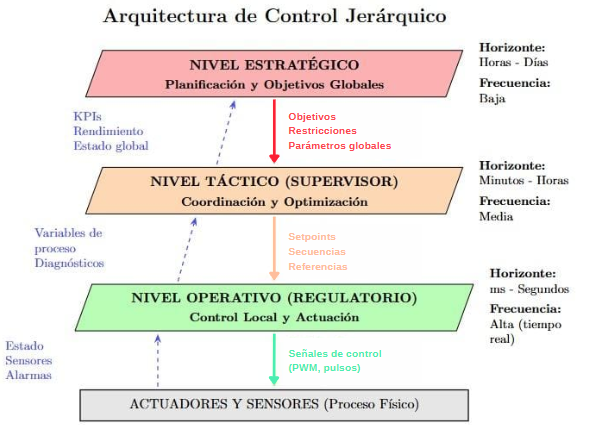
\includegraphics[width=0.8\textwidth]{img/jerarquia_control.png}
    \caption{Estructura piramidal de un sistema de control jerárquico.}
    \label{fig:jerarquia_control}
\end{figure}
La adopción de una arquitectura de control jerárquica ofrece ventajas distintivas que justifican su uso en sistemas complejos:
\begin{itemize}[label=$\bullet$]
    \item \underline{Gestión de la complejidad dimensional}: Permite abordar sistemas de gran escala al descomponer el problema de control multivariable en tareas más simples y manejables a nivel de subsistema.
    \item \underline{Confiabilidad y robustez}: Incrementa la resiliencia operativa, ya que el fallo localizado de un controlador en un nivel inferior solo afecta a un subsistema local, previniendo el colapso de la operación integral de la planta.
    \item \underline{Modularidad y escalabilidad}: Facilita la adición, modificación o reemplazo de subsistemas o unidades de control sin generar un impacto sistémico en el resto de la jerarquía.
    \item \underline{Eficiencia operacional}: Permite la aplicación de diferentes horizontes temporales y estrategias de control especializadas en cada nivel, optimizando tanto la estabilidad (Nivel 1) como la eficiencia global (Niveles 2 y 3).
\end{itemize}